\chapter{Inverted pendulum analysis}


\section{Inverted pendulum description}
For this project an inverted pendulum set up is given. It consists of:
\begin{itemize}
	\item a DC motor
	\item a system of four gears linked by belt strap
	\item an arm
	\item a stick connected to the end of the arm with a liberty of movement of one degree
\end{itemize}

\begin{figure} [htbp]
	\centering
	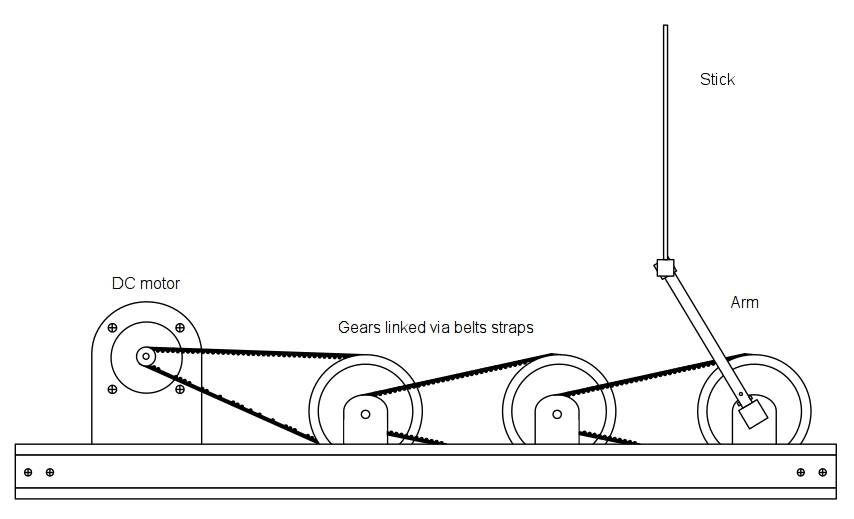
\includegraphics[width=0.8\linewidth]{figures/"Preanalysis&Requirement"/invertedPendulumDiagram}
	\caption{Diagram of the set up fully assembled} \label{fig:InvertedPendulumSetUp}
\end{figure}

\autoref{fig:InvertedPendulumSetUp} is a diagram of the set up when fully assembled. The DC motor moves the arm via the gears, a noteworthy fact is that out the four gears three are of the same size. This means that two gears do not have any influence on the torque and the angular velocity of the arm.

\section{Inverted pendulum modelling}
put the modelling section there